\documentclass[10pt,oneside]{book}

\usepackage{ragged2e}
\usepackage{geometry} 
\usepackage{graphicx}
\usepackage{titlesec}
\usepackage{fontspec}
\usepackage{polyglossia}
\usepackage{epigraph}  % make sure this is loaded
\usepackage{lettrine} % For drop cap
\usepackage{xcolor}
\usepackage{quoting}

\quotingsetup{
  vskip=\baselineskip,
  leftmargin=2em,
  rightmargin=2em,
  font=small
}
\setmainlanguage{hebrew}
\setotherlanguage{english}
\newfontfamily\hebrewfont[Script=Hebrew,Scale=MatchLowercase]{Frank Ruhl Libre}

\geometry{
    paperwidth=107mm,
    paperheight=181mm,
    top=20mm,       % distance from top edge to text
    bottom=16mm,    % distance from bottom edge to text
    left=16mm,
    right=16mm,
    headheight=6mm, % height of the header
    headsep=3mm,    % space between header and text
    footskip=6mm    % distance from bottom of text to page number
}

% Chapter formatting without numbers
\titleformat{\chapter}[display]{\normalfont\huge\bfseries}{}{0pt}{\Huge}


\newcommand{\emptypage}{
  \newpage
  \thispagestyle{empty}
  % Optional: add vertical space if needed
  \vspace*{\fill}
  % Optional content here
  \vspace*{\fill}
  \newpage
}

\newcommand{\hebrewchapter}[2]{%
  \chapter*{#1}%
  \addcontentsline{toc}{chapter}{#1}%
  \lettrine[lines=4, lhang=0.1, loversize=0.5, findent=0pt]{\textcolor{gray} #2}{}%
}

\title{\Huge אנטומיה של המדינה}
\author{}
\date{}
% \author{מארי רות'בארד}
% \date{20.02.1925}

\begin{document}

% ===============================
% Full-page cover image
% ===============================
\newgeometry{top=-0.001cm, bottom=0cm, left=0cm, right=0cm} % remove margins
\thispagestyle{empty}
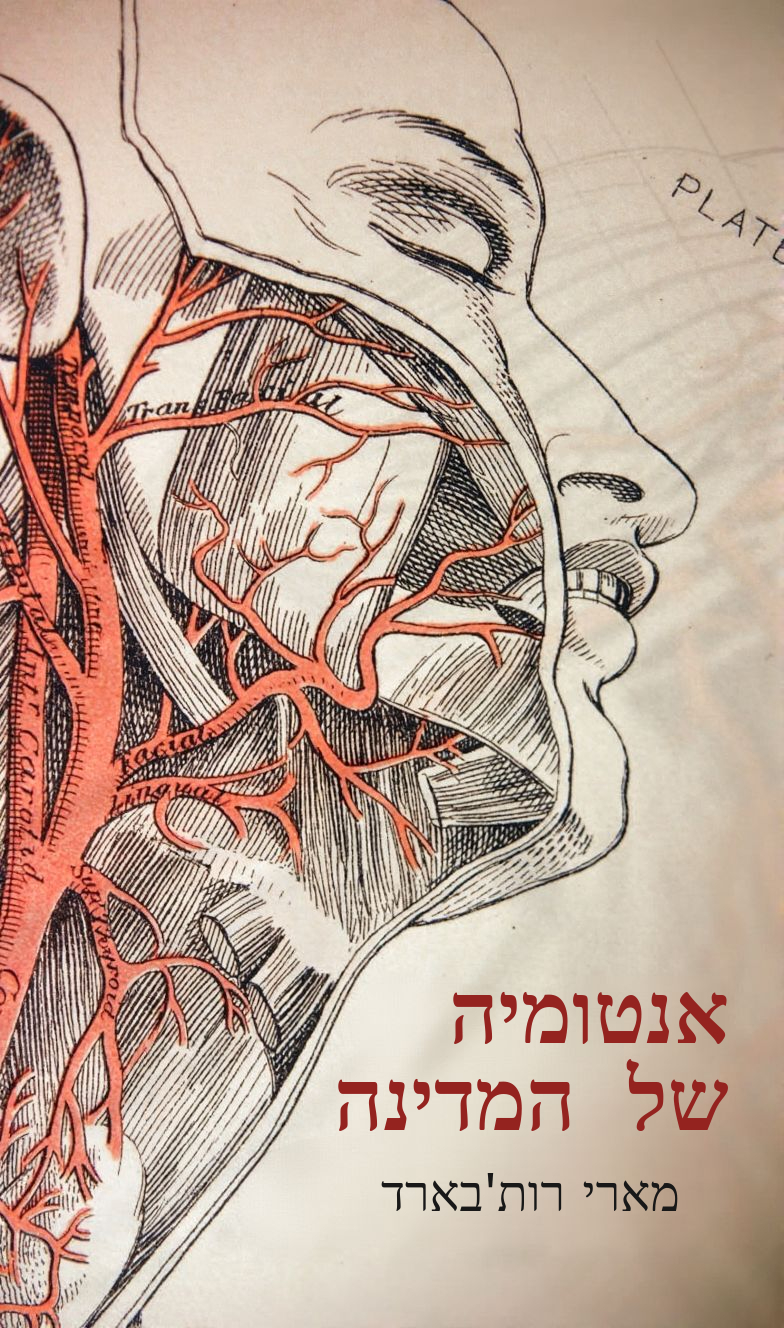
\includegraphics[width=\paperwidth,height=\paperheight]{cover-image.jpg}
\restoregeometry
\newpage

\justifying

% Title page (optional in TOC)
\newpage
\maketitle
\thispagestyle{empty}


%\emptypage

% Quote page
\thispagestyle{empty}
\begin{center}
\vspace*{5cm}
\textit{הסכנה הגדולה ביותר למדינה היא ביקורת אינטלקטואלית עצמאית.} \\
\vspace{1em}
\textbf{מארי רות'בארד}
\end{center}
\newpage


%\emptypage

% ===============================
% Table of contents
% ===============================
\tableofcontents
\newpage

% First chapter
\hebrewchapter{מה המדינה איננה}{ה}
מדינה נחשבת כמעט באופן אוניברסלי ממסד של שירות סוציאלי.
ישנם תיאורטיקנים שמעריצים את המדינה כאפותיאוזה של החברה.
אחרים רואים בו ארגון חביב, אם כי לעתים קרובות לא יעיל, להשגת מטרות חברתיות.
אבל כמעט כולם רואים בה אמצעי הכרחי להשגת מטרות האנושות, אמצעי להתמודד מול המגזר הפרטי ולעתים קרובות לנצח בקרבות על משאבים.
עם עליית הדמוקרטיה, הזיהוי בין המדינה לחברה הוכפל, עד כדי כך שנהוג לשמוע רגשות ודעות המפרות כמעט כל עיקרון של היגיון ושכל ישר, כגון: "אנחנו הממשלה".
המונח הקולקטיבי השימושי "אנחנו" אפשר להטיל הסוואה אידיאולוגית על מציאות החיים הפוליטיים.
אם "אנחנו הממשלה", אז כל מה שממשלה עושה ליחיד אינו רק צודק ולא־עריץ, אלא גם "וולונטרי" מצד אותו יחיד עצמו.
אם הממשלה צברה חוב ציבורי עצום שיש לשלם אותו על ידי מיסוי של קבוצה אחת לטובת קבוצה אחרת, מציאות הנטל מוסתרת באמירה כי "אנחנו חייבים את זה לעצמנו".
אם הממשלה מגייסת אדם בכפייה, או משליכה אותו לכלא בשל דעה חתרנית, הרי שהוא "עושה זאת לעצמו" ולכן לא אירע דבר חמור.
לפי היגיון זה, כל היהודים שנרצחו בידי ממשלת הנאצים לא נרצחו כלל.
במקום זאת, הם "התאבדו", שהרי הם היו הממשלה (שנבחרה באופן דמוקרטי), ולכן כל מה שהממשלה עשתה להם היה וולונטרי מבחינתם.
לא היה עולה על הדעת שיהיה צורך להכביר מילים כדי להדגיש נקודה זו, ובכל זאת רוב עצום של בני האדם מחזיקים בטעות זו במידה רבה או מועטה.

עלינו, אם כן, להדגיש כי "אנחנו" איננו הממשלה.
הממשלה איננה "אנחנו". הממשלה אינה, במובן המדויק, "מייצגת" את רוב העם.
אך אפילו אם כן, אפילו אם 70 אחוז מהאנשים היו מחליטים לרצוח את 30 האחוז הנותרים, עדיין מדובר ברצח ולא בהתאבדות וולונטרית של המיעוט שנרצח.
אין לאפשר לשום מטפורה אורגנית, או לביטוי חסר רלוונטיות כמו "כולנו חלק זה מזה", להסוות עובדה בסיסית זו.

אם, אם כן, המדינה איננה "אנחנו", אם היא איננה "המשפחה האנושית" שמתכנסת כדי לפתור בעיות הדדיות, אם היא איננה מפגש אחווה או מועדון כפרי, מה היא אם כן?
בקצרה, המדינה היא הארגון בחברה שמנסה לשמור על מונופול השימוש בכוח ובאלימות באזור טריטוריאלי מסוים.
בפרט, היא הארגון היחיד בחברה שמקבל את הכנסתו לא דרך תרומה וולונטרית או תשלום עבור שירותים שניתנו, אלא באמצעות כפייה.
בעוד שאנשים או מוסדות אחרים מרוויחים את הכנסתם על ידי ייצור סחורות ושירותים ומכירתם באופן שקט ווולונטרי לאחרים, המדינה מקבלת את הכנסתה באמצעות כפייה.
כלומר, באמצעות השימוש באיום בכלא ובבניית אקדחים או סכינים.
לאחר שהשתמשה בכוח ואלימות כדי להשיג את הכנסתה, המדינה בדרך כלל ממשיכה להסדיר ולפקח על פעולותיהם האחרות של אזרחיה.
אפשר לחשוב שתצפית פשוטה על כל המדינות לאורך ההיסטוריה והעולם תהיה הוכחה מספקת לטענה זו. אך המיתוס שנמתח זמן רב מעל פעולות המדינה מחייב פירוט נוסף.

\hebrewchapter{מהי המדינה}{ה}
אדם נולד ערום אל העולם, והוא נדרש להשתמש בשכלו כדי ללמוד כיצד להשתמש במשאבים שנתנה לו הטבע, ולהפכם (למשל באמצעות השקעה ב"ון") לצורות ומקומות שבהם ניתן לנצל את המשאבים לשביעות רצונו ולהעלאת רמת חייו. הדרך היחידה שבה יכול האדם לעשות זאת היא על ידי שימוש בשכלו ובאנרגיה שלו כדי להפוך משאבים ל"ייצור" ולהחליף את המוצרים הללו במוצרים שנוצרו על ידי אחרים. האדם גילה כי דרך תהליך ההחלפה ההדדית והוולונטרית, ניתן להגדיל באופן ניכר את התפוקה, ובכך את רמות החיים של כל המשתתפים בהחלפה. הדרך היחידה "הטבעית" עבור האדם לשרוד ולהשיג עושר היא, אם כן, להשתמש בשכלו ובאנרגיה שלו כדי לעסוק בתהליך הייצור וההחלפה.

האדם עושה זאת תחילה על ידי מציאת משאבים טבעיים, ואז על ידי הפיכתם (באמצעות "הכנסת עמליו" אליהם, כפי שלוקה אומר) לרכושו הפרטי, ואחר כך על ידי החלפת רכוש זה ברכוש דומה שנרכש על ידי אחרים. הדרך החברתית שמכתיבות דרישות טבעו של האדם היא, אם כן, דרך "זכויות הקניין" ו"שוק חופשי" של מתנה או החלפה של זכויות כאלה. בדרך זו למדו בני האדם כיצד להימנע מ"שיטות הג'ונגל" של מאבק על משאבים נדירים, שבו אדם א' יכול לרכוש אותם רק על חשבון אדם ב', ובמקום זאת להגדיל את המשאבים באופן עצום באמצעות ייצור והחלפה שקטים והרמוניים.

הסוציולוג הגרמני הגדול פרנץ אופןהיימר הצביע על כך שיש שתי דרכים סותרות לרכישת עושר: האחת היא הדרך של ייצור והחלפה שהוזכרה לעיל, אותה כינה "האמצעים הכלכליים". הדרך השנייה פשוטה יותר, שכן היא אינה דורשת פרודוקטיביות; היא הדרך של השתלטות על סחורות או שירותים של אחרים באמצעות כוח ואלימות. זו היא שיטת ההפקעה החד-צדדית, גניבת רכושם של אחרים. שיטה זו כינה אופןהיימר "האמצעים הפוליטיים" לרכישת עושר.

צריך להיות ברור שהשימוש השקט בשכל ובאנרגיה בייצור הוא הדרך "הטבעית" לאדם: האמצעי לשרידתו ושגשוגו על פני כדור הארץ. צריך להיות ברור גם שהאמצעים הכפייתיים והנצלניים סותרים את החוק הטבעי; הם פרזיטיים, שכן במקום להוסיף לייצור, הם מפחיתים ממנו. ה"אמצעים הפוליטיים" מסיטים את הייצור לאדם או קבוצה פרזיטיים והרסניים; וסטייה זו לא רק מפחיתה את מספר המפיקים, אלא גם מורידה את התמריץ של המפיק לייצר מעבר למחייתו. בטווח הארוך, השודד הורס את מחייתו על ידי הפחתה או חיסול מקור אספקתו. אך לא רק זאת; אפילו בטווח הקצר, הטורף פועל בניגוד לטבעו האמיתי כבני אדם.

אנו נמצאים כעת במצב שבו ניתן לענות ביתר פירוט על השאלה: מהי המדינה? המדינה, במילותיו של אופןהיימר, היא "ארגון האמצעים הפוליטיים"; היא התיעול המוסדר של התהליך הטורפי על שטח נתון. שכן פשע, במקרה הטוב, הוא נקודתי ולא ודאי; הפרזיטיות היא ארעית, וקו החיים הכפייתי והפרזיטי עשוי להיחתך בכל עת על ידי התנגדות הקורבנות. המדינה מספקת ערוץ חוקי, מסודר ומסודר לטריפה של רכוש פרטי; היא הופכת את קיומו של מעמד פרזיטי בחברה לודאי, בטוח ויחסית "שקט". מכיוון שהייצור תמיד חייב להקדים את הטריפה, השוק החופשי קדם למדינה. המדינה מעולם לא נוצרה באמצעות "חוזה חברתי"; היא תמיד נולדה בכיבוש ובניצול. הפרדיגמה הקלאסית הייתה שבט כובש שהפסיק לרגע את שיטת השוד והרצח המסורתית שלו על שבט כובש, כדי להבין כי משך השלל יהיה ארוך ובטוח יותר, והמצב נעים יותר, אם השבט הנכבש יורשה לחיות וליצור, בעוד הכובשים מתיישבים ביניהם כשולטים וגובים מס קבוע מדי שנה.

אחת הדרכים להיווצרות מדינה ניתן להמחיש כך: בגבעות דרום "רוריטניה", חבורת שודדים מצליחה להשיג שליטה פיזית על השטח, ולבסוף ראש השודדים מכריז על עצמו כ"מלך הממשל הריבוני והעצמאי של דרום רוריטניה"; ואם לו ולחבריו יש את הכוח לשמור על שלטון זה לזמן מה – הנה! מדינה חדשה הצטרפה ל"משפחת העמים", ומנהיגי השודדים לשעבר הפכו לאצולה החוקית של הממלכה.

\hebrewchapter{כיצד המדינה משמרת את עצמה}{ב}
רגע שהמדינה מוקמת, הבעיה של קבוצת השלטון או ה"קאסטה" היא כיצד לשמור על שלטונה. בעוד שכוח הוא שיטת הפעולה שלהם, הבעיה הבסיסית והארוכת טווח שלהם היא אידיאולוגית. שכן כדי להמשיך בתפקיד, כל ממשלה (ולא רק ממשלה "דמוקרטית") חייבת לזכות בתמיכתם של רוב הנתינים שלה. יש לשים לב שתמיכה זו אינה חייבת להיות התלהבות פעילה; היא יכולה להיות בהחלט סבילה פסיבית, כאילו לחוק טבע בלתי נמנע. אך תמיכה במובן של קבלת המצב, מכל סוג שהוא, חייבת להתקיים; אחרת המיעוט של שליטי המדינה ייכנע בסופו של דבר לעמידה פעילה של רוב הציבור. מכיוון שהטריפה חייבת להיות נתמכת מעודפי הייצור, נכון שהכיתה שמרכיבה את המדינה — הבירוקרטיה במשרה מלאה (והאצולה) — חייבת להיות מיעוט קטן יחסית בארץ, אם כי כמובן ניתן לרכוש בעלי ברית בקרב קבוצות חשובות באוכלוסייה. לכן, המשימה העיקרית של השליטים היא תמיד להבטיח את הקבלה הפעילה או הסבילה של רוב האזרחים.

כמובן, אחת הדרכים להשגת תמיכה היא באמצעות יצירת אינטרסים כלכליים מובנים. לכן, המלך לבדו אינו יכול לשלוט; עליו להיות לו קבוצה ניכרת של תומכים שנהנים מקדימות השלטון, כגון חברי מכשיר המדינה, כמו הבירוקרטיה במשרה מלאה או האצולה המוסדרת. אך גם זאת מבטיחה רק מיעוט של תומכים נלהבים, ואף רכישת התמיכה באמצעות סובסידיות והענקת זכויות מיוחדות אינה מבטיחה את הסכמת הרוב. כדי לקבל את ההסכמה המהותית הזו, יש לשכנע את הרוב באמצעות אידיאולוגיה שהממשלה שלהם טובה, חכמה, ולפחות בלתי נמנעת, ובוודאי טובה יותר מכל חלופה אפשרית אחרת. קידום אידיאולוגיה זו בקרב העם הוא המשימה החברתית החשובה של "האינטלקטואלים". שכן המוני האנשים אינם יוצרים את רעיונותיהם עצמם, ואינם חושבים עליהם באופן עצמאי; הם פועלים באופן פסיבי לפי הרעיונות שמאמצת ומפיצה קבוצת האינטלקטואלים. האינטלקטואלים הם, אם כן, "יוצרי הדעה" בחברה. ומכיוון שהמדינה זקוקה בדיוק לעיצוב דעה כזה, הבסיס לברית עתיקת יומין בין המדינה לאינטלקטואלים ברור.

ברור שהמדינה זקוקה לאינטלקטואלים; לא ברור מדוע האינטלקטואלים זקוקים למדינה. בפשטות, ניתן לומר כי מחייתו של האינטלקטואלי בשוק החופשי אינה יציבה במיוחד; שכן האינטלקטואלי חייב להסתמך על הערכים והבחירות של ההמונים, והמאפיין הבולט של ההמונים הוא שהם בדרך כלל אינם מתעניינים בעניינים אינטלקטואליים. המדינה, לעומת זאת, מוכנה להציע לאינטלקטואלים משרה יציבה וקבועה במכשיר המדינה; וכך הכנסה בטוחה והילה של יוקרה. שכן האינטלקטואלים יזכו לתגמול נאה על התפקיד החשוב שהם מבצעים עבור שליטי המדינה, שהפכו עכשיו להיות חלק מהם.

הברית בין המדינה לאינטלקטואלים סימלה את רצונם הנלהב של פרופסורים באוניברסיטת ברלין במאה התשע-עשרה להקים את "שומרי הראש האינטלקטואליים של בית הוהנצולרן". כיום, ראוי לציין את דבריו המחשמלים של חוקר מרקסיסטי נכבד בנוגע למחקר הביקורתי של פרופסור ויטפוגל על דספוטיזם מזרחי עתיק: "הציוויליזציה שעליה תוקף פרופסור ויטפוגל כל כך בחריפות הייתה כזו שיכלה להפוך משוררים וחוקרים לפקידים." דוגמה נוספת היא התפתחותו האחרונה של תחום "המדע" של אסטרטגיה, בשירות זרוע האלימות המרכזית של הממשלה, הצבא. מוסד ותיק נוסף הוא ההיסטוריון הרשמי או "של החצר", שמוקדש להפצת דעות השליטים על מעשיהם ומעשיהם של קודמיהם.

טיעונים רבים ומגוונים שימשו את המדינה ואת האינטלקטואלים שלה כדי לשכנע את נתיניהם לתמוך בשלטונם. באופן בסיסי, ניתן לסכם את קווי הטיעון כך: (א) שליטי המדינה הם אנשים גדולים וחכמים (הם "שולטים בזכות אלוהית", הם "האצולה" של האנשים, הם "המומחים המדעיים"), גדולים וחכמים בהרבה מהנתינים הטובים אך הפשוטים למדי, ו-(ב) שלטון על ידי הממשלה הוא בלתי נמנע, הכרחי בהחלט, וטוב בהרבה מאלה שמתרחשים אם הוא יפול. האיחוד בין הכנסייה למדינה היה אחד מההתקנים האידיאולוגיים העתיקים והמוצלחים ביותר. השליט הומלך על ידי אלוהים או, במקרה של שלטון מוחלט בדספוטיזם מזרחי, היה הוא עצמו אלוהים; ולכן, כל התנגדות לשלטונו הייתה חילול. הכמורה של המדינה ביצעה את התפקיד האינטלקטואלי הבסיסי של השגת תמיכת הציבור ואפילו פולחן כלפי השליטים.

מכשיר מוצלח נוסף היה להשרות פחד מכל מערכת חלופית של שלטון או אי-שלטון. הובטח שהשליטים הנוכחיים מספקים לאזרחים שירות חיוני שעליהם להוקירו: הגנה מפשע נקודתי ושודדים. שכן המדינה, לשמור על מונופול הטריפה שלה, דאגה שהפשע הפרטי והלא-מוסדר יישמר למינימום; המדינה תמיד הייתה קנאית לשטחה שלה. במיוחד הצליחה המדינה במאות האחרונות לגרום לפחד משלטונות אחרים. מכיוון ששטחי העולם חולקו בין מדינות מסוימות, אחד מעקרונות המדינה היה להזדהות עם השטח שהיא שולטת בו. מאחר שרוב האנשים נוטים לאהוב את מולדתם, ההזדהות עם האדמה ואנשיה הייתה אמצעי להטמעת פטריוטיזם טבעי לטובת המדינה. אם "רוריטניה" הותקפה על ידי "וולדביה", המשימה הראשונה של המדינה ואינטלקטואליה הייתה לשכנע את תושבי רוריטניה שההתקפה היא עליהם ולא רק על הקאסטה השלטת. כך הפכה מלחמה בין שליטים למלחמה בין עמים, כאשר כל עם מגונן על שליטיו באמונה מוטעית שהם מגנים עליו. מנגנון זה של "לאומיות" הצליח רק במאות האחרונות במערב; בעבר הרחוק המוני הנתינים ראו במלחמות קרבות חסרי חשיבות בין קבוצות אצילים שונות.

נשק אידיאולוגי רב-גוני והסודי שימש את המדינה לאורך הדורות. אחד הנשקים היעילים היה המסורת. ככל ששלטון המדינה נשמר זמן רב יותר, כך היה נשק זה חזק יותר; שכן אז לשושלת X או למדינה Y היה המשקל הנראה של מאות שנות מסורת מאחוריה. פולחן אבות, אם כן, הפך לאמצעי ברור להוקרת השליטים הקדומים. הסכנה הגדולה ביותר למדינה היא ביקורת אינטלקטואלית עצמאית; אין דרך טובה יותר לדכא ביקורת זו מאשר לתקוף כל קול מבודד, כל מעורר ספקות חדשים, כמי שחילל את חכמת אבותיו. כוח אידיאולוגי נוסף הוא להמעיט בערכו של הפרט ולהאדיר את הקולקטיב של החברה. שכן כל שלטון מסוים דורש קבלת רוב, וכל סכנה אידיאולוגית יכולה לנבוע רק מפרט או מעטים החושבים באופן עצמאי. רעיון חדש, ובוודאי רעיון ביקורתי חדש, מתחיל בהכרח כמיעוט קטן; לכן המדינה חייבת לדכא דעה זו מיד על ידי לעג לכל דעה המתנגדת לדעת ההמון. "הקשיבו רק לאחיכם" או "התאימו את עצמכם לחברה" הופכים לכלי אידיאולוגי לדיכוי מחלוקת פרטנית. בדרך זו, ההמונים לעולם לא ילמדו על היעדר בגדי הקיסר.

כמו כן, חשוב שהמדינה תגרום לשלטונה להיראות בלתי נמנע; גם אם שלטונה לא נאה, הוא ייתקל בקבלה פסיבית, כפי שמוכיח הביטוי הידוע "מוות ומס". שיטה אחת היא להטמיע דטרמיניזם היסטורי, בניגוד לחירות הרצון של הפרט. אם שושלת X שולטת בנו, זה משום שחוקי ההיסטוריה הבלתי ניתנים לעקיפה (או רצון האל, או הכוח האבסולוטי, או הכוחות הייצוריים החומריים) קבעו כך, ואין דבר שכל פרט קטן יכול לשנות. חשוב גם שהמדינה תטמיע בנתיניה סלידה מכל "תיאוריית קונספירציה היסטורית"; חיפוש "קונספירציות" פירושו חיפוש מניעים והטלת אחריות על מעשים רעים היסטוריים. אם, לעומת זאת, עריצות המדינה, שחיתות או מלחמה תוקפנית נגרמו לא על ידי שליטי המדינה אלא על ידי "כוחות חברתיים" מסתוריים ועתיקים, או על ידי מצב העולם הלקוי או אם באופן כלשהו כולם היו אחראים ("כולנו רוצחים", טוען סיסמה אחת), אין טעם שהציבור יתקומם או יזדעזע. יתר על כן, מתקפה על "תיאוריות קונספירציה" הופכת את הנתינים לפגיעים יותר באמונם בנימוקי "הרווחה הכללית" שהמדינה מציגה עבור פעולותיה העריצות. "תיאוריית קונספירציה" יכולה לערער את המערכת על ידי פקפוק הציבור בתעמולה האידיאולוגית של המדינה.

שיטה נוספת ומוכחת להטיית נתינים לרצון המדינה היא יצירת אשמה. כל עלייה ברווחה הפרטית יכולה להיות מותקפת כ"חמדנות בלתי מצפונית", "חומרנות" או "שפע מוגזם"; רווחים יכולים להיות מותקפים כ"ניצול" ו"ריבית", חילופים הדדיים מותקפים כ"אגואיזם", ובסופו של דבר נובע תמיד המסקנה שעל יותר משאבים להיות מוסטים מהפרטי לציבורי. האשמה המושרת עושה את הציבור מוכן יותר לכך. שכן בעוד שאנשים נוטים לפנק את עצמם ב"חמדנות אגואיסטית", כישלון של שליטי המדינה לעסוק בחילופים אמור להעיד על מסירותם למטרות גבוהות ואצילות — הטריפה הפרזיטית נראית, לכאורה, מוסרית ואסתטית לעומת עבודה שקטה ופרודוקטיבית.

בעידן החילוני יותר של היום, הזכות האלוהית של המדינה הושלמה על ידי קריאה לאל חדש – המדע. שלטון המדינה מוכרז כיום כעל-מדעי, כתכנון על ידי מומחים. אך בעוד ש"ההיגיון" מוזכר יותר מאשר במאות קודמות, זה אינו ההיגיון האמיתי של הפרט ותרגול חירותו; הוא עדיין קולקטיביסטי ודטרמיניסטי, עדיין מתייחס לאגרגטים הוליסטיים ולמניפולציה כפייתית של נתינים פסיביים על ידי שליטיהם.

שימוש גובר בז'רגון מדעי איפשר לאינטלקטואלים של המדינה לרקום אפולוגטיקה מסתורית לשלטון המדינה, שהציבור של עידן פשוט היה מתייחס אליה בזלזול. שודד שהצדיק את גנבתו באמירה שהוא עוזר באמת לקורבנותיו, כי ההוצאות שלו מגבירות את המסחר הקמעונאי, היה מוצא מעט ממירים; אך כאשר תיאוריה זו נתפסת במונחים של משוואות קיינסיאניות ובאזכורים מרשימים ל"אפקט הכפל", היא, למרבה הצער, משכנעת יותר. וכך מתקדם ההתקפה על השכל הישר, כאשר כל דור מבצע את המשימה בדרכו שלו.

מכיוון שתמיכה אידיאולוגית חיונית למדינה, עליה לנסות ללא הרף להרשים את הציבור ב"לגיטימיות" שלה, כדי להבחין בין פעולותיה לבין פעולות של שודדים רגילים. ההחלטיות הבלתי מתפשרת של מתקפותיה על השכל הישר אינה מקרית, שכן, כפי שמחזק מנקן בתיאורים חיים: \\

\begin{quoting}
האדם הממוצע, לא משנה מה טעויותיו אחרת, לפחות רואה בבירור שהממשלה היא משהו שמחוץ לו ומחוץ לרוב בני האדם – שהיא כוח נפרד, עצמאי ועוין, שבשליטתו חלקית בלבד, ויכולה להזיק לו מאוד. האם זה לא מובן מאליו ששוד הממשל נחשב בכל מקום לפשע קטן יותר משוד אדם פרטי, או אפילו תאגיד? ... מה שמאחורי כל זה, אני מאמין, הוא תחושה עמוקה של עוינות בסיסית בין הממשלה לבין האנשים שהיא שולטים בהם. היא נתפסת, לא כוועדת אזרחים שנבחרה לנהל את ענייני הכלל, אלא כישות נפרדת ואוטונומית, העוסקת בעיקר בניצול האוכלוסייה לטובת חבריה בלבד... כאשר אזרח פרטי נבזז, אדם ראוי מאבד את פירות עבודתו וחסכונותיו; כאשר הממשלה נבזזה, הגרוע ביותר שמתרחש הוא שכמה רמאים וטפילים יש להם פחות כסף לשחק איתו מאשר קודם. הרעיון שהם הרוויחו את הכסף הזה לעולם אינו נשקל; לרוב האנשים הסבירים זה היה נראה מגוחך.
\end{quoting}

\hebrewchapter{כיצד חורגת המדינה מגבלותיה}{כ}
פי שברטרנד דה ז'ובנל העיר בחוכמה, במשך המאות בני אדם יצרו מושגים שנועדו לבדוק ולהגביל את מימוש שלטון המדינה; ואולם, אחד אחרי השני, הצליחה המדינה, באמצעות בני ברית אינטלקטואלים שלה, להפוך את המושגים הללו ל"מחותמות גומי" של לגיטימציה ומעלה, שניתן להדביק על צווים ופעולותיה. במקור, במערב אירופה, מושג הריבונות האלוהית קבע שהמלכים יכולים לשלוט אך ורק בהתאם לחוק האלוהי; המלכים הפכו את המושג למותג של אישור אלוהי לכל פעולה שלהם. מושג הדמוקרטיה הפרלמנטרית החל כבדיקה עממית כנגד שלטון מלוכני מוחלט; בסופו של דבר, הפך הפרלמנט לחלק חיוני מהמדינה וכל פעולתו ריבונית לחלוטין. כפי שמסכם דה ז'ובנל:

\begin{quoting}
"רבים מהכותבים על תיאוריות ריבונות פיתחו אחת... מהאמצעים המגבילים הללו. אך בסופו של דבר כל אחת מהתיאוריות הללו איבדה, מוקדם או מאוחר, את מטרתה המקורית, והפכה למקפצה לכוח, בכך שסיפקה לו את הסיוע החזק של ריבון בלתי נראה עם אשר יוכל להזדהות עמו בהצלחה עם הזמן."
\end{quoting}

דבר דומה מתרחש עם דוקטרינות יותר ספציפיות: "הזכויות הטבעיות" של הפרט, כפי שמובאות בכתביו של ג'ון לוק ובמגילת הזכויות, הפכו ל"זכות סטטיסטית לעבודה"; תועלתנות הפכה מארגומנטים בעד חירות לארגומנטים נגד התנגדות לפלישות המדינה לחירות, וכדומה.

הניסיון השאפתני ביותר להגביל את המדינה היה מגילת הזכויות וחלקים מגבילים אחרים של החוקה האמריקאית, שבהם גבולות כתובים לממשל הפכו לחוק יסוד שצריך להיות מפורש על ידי מערכת שיפוטית שנחשבת עצמאית משאר סניפי הממשל. כל האמריקאים מכירים את התהליך שבו פירוש הגבולות בחוקה הורחב בעקביות במהלך המאה האחרונה. אך מעטים שמו לב, כמו הפרופסור צ'ארלס בלק, לכך שהמדינה הפכה למעשה את הביקורת השיפוטית עצמה מכלי מגביל לכלי נוסף להענקת לגיטימציה אידיאולוגית לפעולות הממשלה. שכן אם צו שיפוטי המכריז "לא חוקתי" מהווה בדיקה עוצמתית לכוח הממשלתי, הכרזה משתמעת או מפורשת של "חוקתי" היא נשק חזק לטיפוח קבלת הציבור לכוח ממשלתי הולך וגדל.

בלק מתחיל את ניתוחו בהדגשת הצורך הקריטי ב"לגיטימציה" כדי שממשל יתקיים, לגיטימציה זו מציינת קבלת רוב בסיסית של הממשלה ופעולותיה. קבלת לגיטימציה היא בעיה מיוחדת במדינה כמו ארצות הברית, שבה "מגבלות מהותיות מובנות בתיאוריה שעל פיה מושתת הממשל". מה שנדרש, מוסיף בלק, הוא אמצעי להבטיח לציבור שכוחות הממשל ההולכים וגדלים אכן "חוקתיים". והוא מסכם כי זו הייתה תפקידה ההיסטורי העיקרי של הביקורת השיפוטית.

בלק מדגים את הבעיה:

\begin{quoting}
"הסיכון העליון [לממשל] הוא תחושת אי-סיפוק וזעם המופץ ברבים באוכלוסייה, ואובדן הסמכות המוסרית של הממשלה ככזו, לא משנה כמה זמן היא נתמכת בכפייה או אינרציה או בחוסר חלופה מושכת ומיידית. כמעט כל מי שחי תחת ממשל מוגבל חייב מוקדם או מאוחר להיות נתון לפעולה ממשלתית שהוא רואה כחורג מסמכות הממשל או אפילו אסורה עליו. אדם מגויס לצבא, למרות שאינו מוצא דבר בחוקה על גיוס חובה... חקלאי מונחה כמה חיטה לגדל; הוא מאמין, ומגלה שכמה עורכי דין מכובדים מסכימים עמו, שהממשלה אינה רשאית להורות לו כמה חיטה לגדל יותר מאשר להורות לבתו עם מי היא יכולה להינשא. אדם נכנס לכלא פדרלי על אמירת מה שהוא רוצה, והוא מסתובב בתאו ומספר לעצמו... 'הקונגרס לא יעשה חוקים המגבילים את חופש הדיבור'... איש עסקים מונחה מה הוא יכול לבקש וחייב לבקש עבור מחלב."
\end{quoting}

הסיכון הוא אמיתי, שכל אחד מהאנשים הללו (ומי לא ביניהם?) יתמודד עם מושג המגבלות הממשלתיות מול המציאות כפי שהוא תופס אותה, ויגזור מסקנה לגבי לגיטימיות ממשלו.

סיכון זה נמנע על ידי הצגת הדוקטרינה שהסמכות האחרונה לפרש את החוקה חייבת להיות סוכנות אחת, ובסופו של דבר חלק מהממשלה הפדרלית. מכיוון שעצמאות השיפוט הפדרלי יוצרת את פעולותיו כאילו הן "כתובים קדושים" עבור רוב הציבור, גם נכון תמיד שהמערכת השיפוטית היא חלק ממנגנון הממשלה וממונה על ידי הסניפים המבצעים והמחוקקים. בלק מודה שזה אומר שהמדינה שמה את עצמה כשופטת בתיק שלה עצמו, ובכך מפרה עקרון משפטי בסיסי של צדק בהחלטות.

בלק מוסיף:

\begin{quoting}
"הבעיה, אם כן, היא להמציא אמצעים ממשלתיים להחלטה כך שיופחתו למינימום סביר את עוצמת ההתנגדות לכך שהממשלה היא השופטת בתיק שלה. לאחר מכן, ניתן רק לקוות שההתנגדות תאבד מהכוח שלה, כדי שהעבודת הלגיטימציה של מוסד ההחלטה תזכה בקבלה."
\end{quoting}

בסופו של דבר, בלק רואה בהשגת צדק ולגיטימציה מתוך בחינת המדינה את תיקיה כ"מעין נס".

ביישום תיאוריה זו למאבק המפורסם בין בית המשפט העליון לניו דיל, בלק מגנה על חבריו התומכים בניו דיל על חוסר ראייתם קדימה בכך שהם מגנים את ההתנגדות השיפוטית:

\begin{quoting}
"גרסת הסיפור הסטנדרטית על ניו דיל והבית המשפט, אף שהיא נכונה במידה מסוימת, מסירה את הדגש... היא מתמקדת בקשיים; כמעט שוכחת איך הכל הסתיים. התוצאה הייתה, לאחר כעשרים וארבעה חודשים של התנגדויות... בית המשפט העליון, בלי שינוי אחד בחוק הרכבו או בהרכב בפועל, העניק חותמת חיובית של לגיטימציה על ניו דיל, ועל התפיסה החדשה כולה של ממשל באמריקה."
\end{quoting}

כך, בית המשפט העליון הצליח להרגיע את רוב האמריקאים שהיו להם התנגדויות חוקתיות חזקות לניו דיל:

\begin{quoting}
"כמובן, לא כולם היו מרוצים. אך אין עוד ספק ציבורי משמעותי או מסוכן לגבי סמכות חוקתית של הקונגרס לטפל כפי שהוא עושה בכלכלה הלאומית..."
\end{quoting}

ללא בית המשפט העליון לא היה לנו אמצעי אחר להענקת לגיטימציה לניו דיל. כפי שמכיר בלק, אחד התיאורטיקנים הפוליטיים המרכזיים, ג'ון סי. קלקון, הבין מראש את החור הבולט במגבלות חוקתיות של הממשלה: מינוי סמכות פרשנית סופית לבית המשפט העליון. קלקון הציע את דוקטרינת הרוב המקביל ("concurrent majority"): אם מיעוט משמעותי במדינה, למשל ממשלת מדינה, סבור שהממשל הפדרלי חורג מסמכויותיו, למיעוט זה יש זכות להטיל וטו על פעולה זו כבלתי חוקתית.

לסיכום, המדינה תמיד הראתה כישרון יוצא דופן להרחיב את סמכויותיה מעבר לכל מגבלה שהטילו עליה. מאחר שהמדינה חייבת להתקיים על בסיס החרמת הון פרטי, והרחבתה כרוכה בפגיעות גדלות בפרט ובעסקים פרטיים, עלינו לקבוע שהמדינה אנטי-קפיטליסטית במהותה. למעשה, לעומת הטענה המרקסיסטית שהמדינה היא "ועדת הביצוע" של מעמד השלטון (לכאורה הקפיטליסטים), המדינה עצמה היא מקור ומרכיב המעמד השולט (הקסטה השלטת), וניצבת תמיד מול ההון הפרטי. דה ז'ובנל מסכם:

\begin{quoting}
"רק מי שאינו יודע דבר על שום תקופה מלבד זמנו שלו, וחשוך לחלוטין לגבי התנהגות הכוח במשך אלפי שנים, יראה במהלכים אלו [הלאומיים, מס הכנסה וכו'] את פירות דוקטרינות מסוימות. הם למעשה ביטויים נורמליים של כוח, ואינם שונים במהותם מהחרמות המנזרים על ידי הנרי השמיני. אותו עקרון פועל; הרעב לסמכות, הצמא למשאבים; ובכל הפעולות הללו מופיעים אותם מאפיינים, כולל העלייה המהירה של המחלקים של השלל. בין אם מדובר בסוציאליסט או לא, הכוח יהיה תמיד במלחמה עם הרשויות הקפיטליסטיות ויחרים את הון הקפיטליסטים; בכך הוא מציית לחוק טבעו."
\end{quoting}

\hebrewchapter{ממה המדינה חוששת}{מ}
ה שהמדינה חוששת ממנו מעל לכל, כמובן, הוא כל איום יסודי על כוחה ועל קיומה. מותה של מדינה יכול להתרחש בשתי דרכים עיקריות: (א) על ידי כיבוש על ידי מדינה אחרת, או (ב) על ידי הפיכה מהפכנית בידי נתיניה—בקיצור, על ידי מלחמה או מהפכה. מלחמה ומהפכה, כשני האיומים הבסיסיים, מעוררים אצל שליטי המדינה את המאמצים המרביים ואת התעמולה המרבית בקרב העם. כפי שנאמר לעיל, יש תמיד להשתמש בכל דרך כדי למצות את העם ולהניע אותו להגן על המדינה באמונה שהם מגנים על עצמם. שגיאת הרעיון נעשית ברורה כאשר גיוס בכפייה מופעל נגד אלה המסרבים "להגן" על עצמם ונאלצים, לפיכך, להצטרף לזרוע הצבאית של המדינה: מיותר לציין, כי לא מותרים להם שום "הגנה" נגד מעשה זה של "מדינתם".

במלחמה, כוח המדינה נדחף לקיצו, ותחת סיסמאות של "הגנה" ו"חירום" ניתן להטיל עריצות על הציבור שאולי הייתה נתקלת בהתנגדות גלויה בשעת שלום. המלחמה מספקת, אם כן, יתרונות רבים למדינה, ואכן כל מלחמה מודרנית הביאה עם עצמה לאוכלוסייה הלוחמת מורשת קבועה של עול מדינתי מוגבר על החברה. יתר על כן, מלחמה מספקת למדינה הזדמנויות מפתות לכיבוש שטחי אדמה שבהם היא יכולה לממש את מונופול הכוח שלה. רנדולף בורן צדק בהחלט כשכתב ש"מלחמה היא בריאותה של המדינה", אך עבור כל מדינה מסוימת מלחמה עשויה להכתיב בריאות או פגיעה חמורה.

ניתן לבחון את ההשערה שהמדינה מעוניינת בעיקר להגן על עצמה ולא על נתיניה על ידי שאילת השאלה: איזו קטגוריה של פשעים המדינה מרדפת ומענישה באופן החמור ביותר—אלה נגד אזרחים פרטיים או אלה נגד עצמה? הפשעים החמורים ביותר במילון המדינה כמעט תמיד אינם פלישות לאדם או רכוש פרטי, אלא סכנות לנוחיותה שלה, לדוגמה: בגידה, עריקות חייל לאויב, כישלון ברישום לגיוס, הפיכה וקונספירציה תת-סודית, רצח של שליטים ופשעים כלכליים נגד המדינה כגון זיוף מטבעה או התחמקות ממס הכנסה. או להשוות את מידת ההתלהבות ברדיפת אדם המכה שוטר, עם תשומת הלב שהמדינה מעניקה למתקפה על אזרח רגיל. ואולם, באופן מעניין, הקדימות הפומבית שהמדינה מעניקה להגנתה מפני הציבור נדמית למעטים כסותרת את הייעוד המניחים לה.


\hebrewchapter{כיצד מדינות מתייחסות זו לזו}{מ}
כיוון ששטח כדור הארץ מחולק בין מדינות שונות, יחסים בין-מדינתיים חייבים לתפוס חלק ניכר מזמנם ומאנרגייתם של המדינות. הנטייה הטבעית של מדינה היא להרחיב את כוחה, ובחוץ זה מתרחש בדרך כלל על ידי כיבוש שטח טריטוריאלי. אלא אם כן השטח חסר מדינה או בלתי מאוכלס, כל התרחבות כזו כרוכה בקונפליקט אינטרסים מהותי בין קבוצה אחת של שליטי מדינה לאחרת. רק קבוצה אחת של שליטים יכולה להשיג מונופול על כפייה בכל שטח טריטוריאלי מסוים בכל רגע נתון: כוח מלא על שטח על ידי מדינה X ניתן להשגה רק על ידי גירוש מדינה Y. מלחמה, אף שהיא מסוכנת, תהיה נטייה תמידית של מדינות, המתחלפת בתקופות שלום ובבריתות והקואליציות המשתנות בין המדינות.

ראינו כי הניסיון ה"פנימי" או "ביתי" להגביל את המדינה במאות ה-17 עד ה-19 הגיע לצורתו המובהקת ביותר בצורת הממשל החוקתי. מקבילו ה"חיצוני" או "בעניין יחסי חוץ" היה פיתוח "החוק הבינלאומי", במיוחד בצורות כמו "דיני מלחמה" ו"זכויות נייטרליות". חלקים מהחוק הבינלאומי היו במקור פרטיים לחלוטין, וצמחו מתוך הצורך של סוחרים וטריידרים בכל מקום להגן על רכושם וליישב סכסוכים. דוגמאות לכך הן דיני אדמירליות וחוק הסוחר. אך אפילו הכללים הממשלתיים צמחו באופן וולונטרי ולא הוטלו על ידי על-מדינה בינלאומית כלשהי. מטרת "דיני המלחמה" הייתה להגביל את ההרס הבין-מדינתי רק למנגנון המדינה עצמו, ובכך להגן על הציבור האזרחי התמימים מפני הקטל והחורבן של המלחמה. מטרת פיתוח זכויות הנייטרלים הייתה לשמור על מסחר אזרחי בינלאומי פרטי, גם עם מדינות "אויבות", מפני החרמה על ידי אחת המפלגות הלוחמות. המטרה העליונה, אם כן, הייתה להגביל את היקף המלחמה, ובפרט להגביל את השפעתה ההרסנית על האזרחים הפרטיים של המדינות הנייטרליות ואפילו של המדינות הלוחמות.

המשפטן F.J.P. Veale מתאר בכיף את מהלך "המלחמה המתרבת" כפי שהתקיימה בקצרה באיטליה במאה ה-15:

\begin{quoting}
הבורגרים והסוחרים העשירים של ימי הביניים באיטליה היו עסוקים מדי בכסף ובהנאות החיים כדי לעסוק בעצמם בקשיי וסכנות הלחימה. לכן הם אימצו את הנוהג לשכור שכירי חרב להילחם במקומם, וכיוון שהיו אנשים חסכנים ומעשיים, פיטרו את שכירי החרב מיד לאחר שהשירות שלהם הסתיים. מלחמות, אם כן, נוהלו על ידי צבאות שכירי חרב לכל מסע מלחמה. . . . בפעם הראשונה, החיילות הפכה למקצוע הגיוני וביחסית בלתי מזיק. הגנרלים של אותה תקופה ניהלו את המהלכים זה נגד זה במיומנות רבה, אך כאשר אחד השיג יתרון, יריבו בדרך כלל או נסוג או נכנע. היה כלל מוכר כי עיר יכולה להיות נשדדת רק אם היא הציעה התנגדות: חסינות תמיד ניתנת לרכישה בתשלום כופר. . . . כתוצאה טבעית, אף עיר לא התנגד, שכן ברור שממשל חלש מדי להגן על אזרחיו איבד את נאמנותם. לאזרחים היה מעט מה לחשוש מסכנות המלחמה שהיו עניינם של חיילים מקצועיים בלבד.
\end{quoting}

ההפרדה כמעט מוחלטת בין האזרח הפרטי לבין מלחמות המדינה באירופה במאה ה-18 מודגשת על ידי נף:

\begin{quoting}
אפילו התקשורת הדוארית לא הוגבלה בהצלחה לאורך זמן בזמן מלחמה. מכתבים הסתובבו ללא צנזורה, בחופשיות שהפתיעה את המחשבה של המאה ה-20. . . . נתיני שתי המדינות הלוחמות שוחחו זה עם זה אם נפגשו, וכשלא יכלו להיפגש, הם כתבו זה לזה, לא כאויבים אלא כחברים. הרעיון המודרני כמעט ולא התקיים כי . . . נתיני מדינה אויבים אחראים בחלקם למעשי הלחימה של שליטיהם. ואף השליטים הלוחמים לא היו נוטים לעצור את התקשורת עם נתיני האויב. הפרקטיקות הימי-ביניימיות של ריגול בדת ואמונה נעלמו, ואף חקירה מקבילה בקשר לתקשורת פוליטית או כלכלית אפילו לא נחשבה. דרכונים נוצרו במקור כדי להעניק מעבר בטוח בזמן מלחמה. במשך רוב המאה ה-18, כמעט שלא עלה על הדעת כי האירופים ינטשו את מסעותיהם במדינה זרה שהמדינה שלהם נלחמת בה.
\end{quoting}

ומאחר שהמסחר הוכר יותר ויותר כמועיל לשני הצדדים, המלחמה במאה ה-18 איזנה גם כמות ניכרת של "מסחר עם האויב".

עד כמה המדינות עברו את גבולות המלחמה המתורבתת במאה זו אינו דורש פירוט כאן. בעידן המודרני של מלחמה כוללת, בשילוב עם טכנולוגיה להשמדה כוללת, נראה כי הרעיון עצמו של שמירת המלחמה מוגבלת למנגנון המדינה הוא אפילו יותר מיושן ומוזר מהחוקה המקורית של ארצות הברית.

כאשר המדינות אינן במלחמה, לעיתים יש צורך בהסכמים כדי למנוע חיכוכים ככל האפשר. אחת הדוקטרינות שקיבלה קבלה רחבה באופן מעניין היא הטענה ל"קדושת ההסכמים". רעיון זה מטופל כמקבילה ל"קדושת החוזה". אך חוזה והסכם אין להם דבר במשותף. חוזה מעביר, באופן מדויק, זכויות לרכוש פרטי. מאחר שממשל אינו, בכל מובן ראוי, "בעלים" של שטחו הטריטוריאלי, כל הסכם שהוא חותם אינו מעניק זכויות לרכוש. אם, למשל, מר ג'ונס מוכר או מעניק את אדמתו למר סמית', היורש של ג'ונס אינו יכול לדרוש את האדמה באופן חוקי על פי יורש סמית'. הזכות לרכוש כבר הועברה. החוזה של ג'ונס הקודם מחייב אוטומטית את ג'ונס הצעיר, מכיוון שהקודם כבר העביר את הנכס; ג'ונס הצעיר, לכן, אין לו טענה לרכוש. ג'ונס הצעיר יכול לטעון רק את מה שהוא ירש מג'ונס הישן, וג'ונס הישן יכול להוריש רק את הרכוש שהוא עדיין מחזיק בו. אך אם בתאריך מסוים, ממשלת רוריטניה נאלצת או אפילו מושחתת על ידי ממשלת ולדביה לוותר על חלק משטחה, זה אבסורדי לטעון שממשלות או תושבי שתי המדינות מנועים לנצח מלטעון לאיחוד מחדש של רוריטניה בטענה ל"קדושת ההסכם". לא העם ולא אדמת רוריטניה הצפונית-מערבית שייכים לאחת משתי הממשלות. כתוצאה מכך, ממשלה אחת אינה יכולה לקשור, באמצעות "יד מתה" של העבר, ממשלה מאוחרת יותר דרך הסכם. ממשלה מהפכנית שהפילה את מלך רוריטניה לא הייתה, באופן דומה, יכולה להיות נקראת אחראית לפעולות או חובות המלך, שכן ממשלה אינה, כמו ילד, יורשת אמיתית לרכוש קודמתה.

\hebrewchapter{ההיסטוריה כמרוץ בין כוח המדינה לבין הכוח החברתי}{ב}
דיוק כפי שהיחסים הבסיסיים והבלעדיים בין בני אדם הם שיתוף פעולה שלוּי-שלום או ניצול בכפייה, ייצור או טורפות, כך ניתן לראות את תולדות האנושות, ובמיוחד את תולדותיה הכלכליות, כמאבק בין שני עקרונות אלו. מצד אחד, קיימת פרודוקטיביות יצירתית, החלפה ושיתוף פעולה בשלום; מצד שני, קיימת כפייה ודיקטטורה והטורפות על יחסים חברתיים. אלברט ג'יי נוק כינה בכיף את הכוחות המתחרים הללו: "כוח חברתי" ו"כוח המדינה".

הכוח החברתי הוא כוחו של האדם על הטבע, השינוי שיתוף הפעולה שלו של משאבי הטבע ותובנתו את חוקי הטבע, לטובת כל הפרטים המשתתפים. כוח חברתי הוא הכוח על הטבע, הרמות החיים שהושגו על ידי האדם בהחלפה הדדית. כוח המדינה, כפי שראינו, הוא החריגה הכפויה והטפילית של ייצור זה—שאיבת פירות החברה לטובת שליטים לא-מייצרים (ובפועל אנטי-מייצרים). בעוד שהכוח החברתי פועל על הטבע, כוח המדינה הוא כוח על האדם.

במהלך ההיסטוריה, כוחותיו היצירתיים והפרודוקטיביים של האדם חפרו שוב ושוב דרכים חדשות לשנות את הטבע לטובת האדם. אלו היו הזמנים שבהם הכוח החברתי הקדימה את כוח המדינה, וכאשר מידת חדירת המדינה לחברה הצטמצמה באופן משמעותי. אך תמיד, לאחר פער זמן גדול או קטן, המדינה נכנסה לתחומים החדשים הללו, כדי לשתק ולהחרים את הכוח החברתי פעם נוספת. אם המאות ה-17 עד ה-19 היו, במדינות רבות במערב, תקופות של עלייה בכוח החברתי, ועלייה נלווית בחופש, שלום ורווחה חומרית, המאה ה-20 הייתה בעיקר עידן שבו כוח המדינה רדף אחרי ההתקדמות—עם חזרה נלווית לעבדות, מלחמה והרס.

במאה זו, המין האנושי מתמודד שוב עם שלטון מרושע של המדינה—של מדינה שמצוידת כעת בפירות כוחות היצירה של האדם, שהוחרמו ועוותו למטרותיה שלה. כמה מאות השנים האחרונות היו זמנים שבהם ניסו בני אדם להציב גבולות חוקתיים ואחרים על המדינה, רק כדי לגלות שגבולות אלו, כמו כל ניסיונות אחרים, נכשלו. מכל הצורות הרבות שהממשלות קיבלו במהלך המאות, מכל המוסדות והמוסכמות שניסו, אף אחת לא הצליחה לשמור את המדינה תחת שליטה. הבעיה של המדינה, ככל הנראה, רחוקה מפתרון כמו בעבר. אולי יש לחקור דרכים חדשות, אם אי פעם יושג פתרון סופי ומוצלח לשאלת המדינה.

\end{document}
